%!TEX root = ../proteoform_suite_manual.tex
%---------------------------------------------------------------------
%	THEORETICAL DATABASE
%---------------------------------------------------------------------

\section{Theoretical Database}

\subsection{Overview}
On this page, theoretical proteoforms are created using the file(s) loaded under Protein Databases on the Load Results page. This theoretical proteoform database includes theoretical proteoforms with combinations of annotated post-translational modifications (PTMs) and subsequences. Theoretical proteoforms are used in intact-mass analysis to identify proteoforms (see \textbf{Experiment-Theoretical Comparison} section). Decoy databases are also generated to compute a false discovery rate for intact-mass proteoform identifications. The modifications table (bottom right) enables a user to edit modifications.  The bottom-up result file(s) loaded under MetaMorpheus Bottom-Up Unique Peptides on the Load Results Page is used to create a list of bottom-up peptides, which are integrated with theoretical proteoforms. 

\subsection{Run Page}
\begin{itemize}
\item Load database file(s) on the Load Results page under Protein Databases (see \textbf{Load Results} section)
\item Set all parameters as desired for current analysis (see below)
\item Click Run Page button (top right)
\end{itemize}

\subsection{Set Parameters}
\begin{figure}[h]
\centering
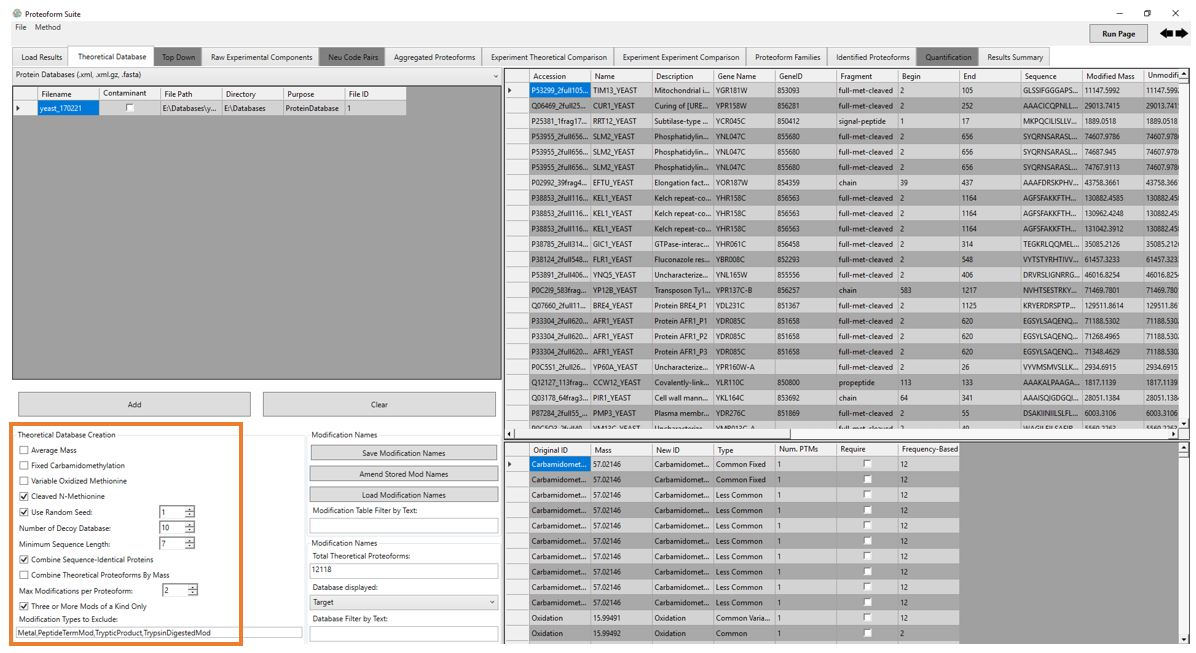
\includegraphics[scale=0.43]{figures/theoretical1.jpg}
\end{figure}
\begin{itemize}
\item Average Mass: if checked, the average mass of each theoretical proteoform will be used instead of the default monoisotopic mass
\item Fixed Carbamidomethylation: if checked, each cysteine on each theoretical proteoform will have a carbamidomethylation group added
\item Variable Oxidized Methionine: if checked, theoretical proteoforms will be added with oxidation modifications up to the number of methionine residues/the Max Modifications per Proteoform parameter setting
\item Cleaved N-Methionine: if checked, methionine will be cleaved off of each full sequence (subsequences UniProt containing the N-methionine will still be added)
\item Use Random Seed: a random seed will be used in the random number generator creating decoy databases, resulting in the same decoy database each time (with the same given parameters)
\item Random Seed: this number will be used for the random seed if the Use Random Seed box is checked
\item Number of Decoy Databases: the number of decoy databases generated. The average across each decoy database result is used to compute the false discovery rate for intact-mass identifications
\item Minimum Sequence Length: the minimum length of a theoretical proteoform in the database
\item Combine Sequence-Identical Proteins: if checked, sequences that are the same from different genes/proteins will be combined into a single theoretical proteoform entry
\item Combine Theoretical Proteoforms by Mass: if checked, different proteoforms with the same mass (up to 4 decimal places) will be combined into a single theoretical proteoform entry
\item Max Modifications per Proteoform: theoretical proteoforms will be generated for each UniProt protein entry containing annotated modifications in different combinations up to this number
\item Three or More Mods of a Kind Only: if checked, modification combinations with different modifications will only go up to 2 modifications per theoretical proteoform. If Max Modifications per Proteoform is set to greater than 2, only modification combinations containing annotated modifications of the same type (ex: triphospho) will go from three modifications up to this number
\item Modification Types to Exclude: comma-separated list of types of modifications to exclude for annotated modifications in the database
\pagebreak
\item Modification Names table: the bottom right table displays each input modification. Several columns can be edited in this table:
\begin{figure}[htbp]
\centering
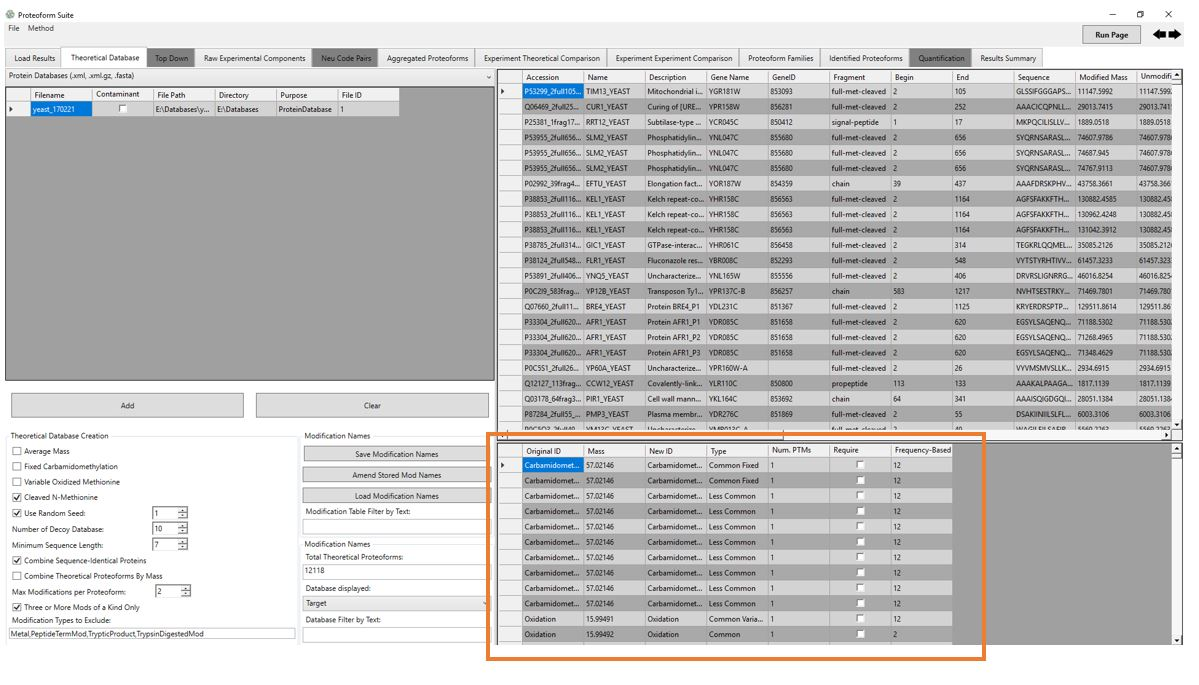
\includegraphics[scale=0.43]{figures/theoretical.jpg}
\end{figure}
\begin{itemize}
\item New ID: the unlocalized version of the modification name, used in Proteoform Suite intact-mass analysis
\item Num. PTMs Represented: the number of PTMs represented by this PTM entry (ex: Dimethylation - 2 PTMs)
\item Require Proteoform Without This Modification: if checked, a proteoform is only identified containing this modification if a proteoform without this modification is also identified. Potentially useful for modifications such as adducts
\item Frequency-Based Rank of PTM Mass: this rank is used in intact-mass analysis to favor more common modifications (lower number is prioritized).
\end{itemize}
\item Save Modification Names: saves a new .modnames file with edits in Modification Names table
\item Amend Stored Mod Names: saves and overwrites .modnames file used in Proteoform Suite
\item Load Modification Names: load a new .modnames file for use in current analysis
\item Modification Table Filter by Text: filter the Modification Names table (bottom right) by any entered text
\end{itemize}

\subsection{Results}

\begin{itemize}
	\item Theoretical Proteoforms table: the top right table displays all theoretical proteoforms generated
	\begin{figure}[h]
\centering
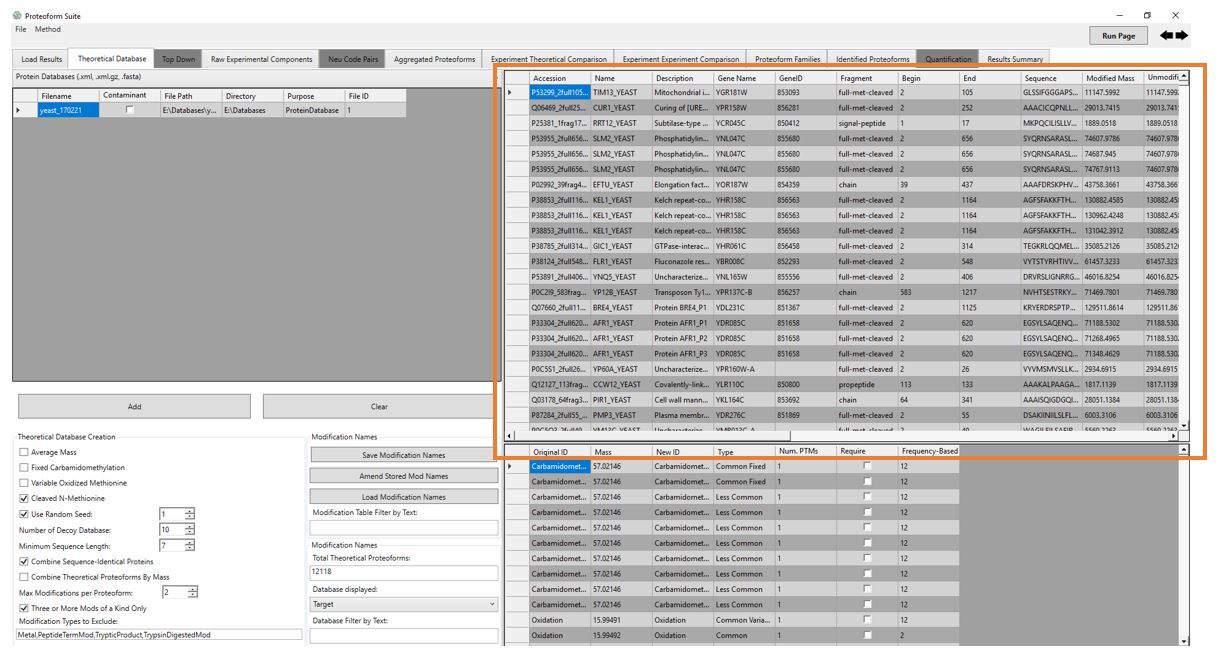
\includegraphics[scale=0.42]{figures/theoretical2.jpg}
\end{figure}
	\begin{itemize}
		\item Accession: accession given by Proteoform Suite for this specific theoretical proteoform
		\item Name: protein name from UniProt
		\item Description: protein description from UniProt
		\item Gene Name: gene name from UniProt
		\item GeneID: gene ID from UniProt
		\item Fragment: sequence description
		\item Begin: theoretical proteoform begin residue in protein full sequence in UniProt
		\item End: theoretical proteoform end residue in protein full sequence in UniProt
		\item Sequence: theoretical proteoform sequence
		\item Modified Mass: monoisotopic (or average) mass of theoretical proteoform with any modifications
		\item Unmodified Mass: monoisotopic (or average) mass of theoretical proteoform without modifications
		\item PTM Mass: mass of PTMs on theoretical proteoform
		\item Contaminant: checked if theoretical proteoform is from contaminant database
		\item Lysine Count: number of lysines in theoretical proteoform sequence
		\item PTM Description: PTMs on theoretical proteoform
		\item GO Term IDs: Gene Ontology term IDs from UniProt
		\item Grouped Accessions: accession grouped if Combine Sequence-Identical Proteins and/or Combine Theoretical Proteoforms By Mass are checked
		\item Top-Down Theoretical: theoretical proteoform identified by top-down analysis (must run Top-Down page first)
		\item Not in Original Database: theoretical proteoform added because of top-down identification, not in original database pre-top-down-analysis (must run Top-Down page first)
		\item Bottom-Up PSMs Count: number of bottom-up PSMs derived from this theoretical proteoform
		\item Peptide-Specific Modified Bottom-Up PSMs: modified residues confirmed ID'd by bottom-up peptides derived from this theoretical proteoform, keeping unique peptidoforms separate
		\item Modified Bottom-Up PSMs: modified residues confirmed by ID'd bottom-up peptides derived from this theoretical proteoform
		\item Bottom-Up Evidence for All PTMs: checked if all PTMs on this theoretical proteoform are confirmed by at least one modified bottom-up peptide
		\item Bottom-Up Evidence for Begin: checked if bottom-up peptide identified with begin residue at this theoretical proteoform's begin residue
		\item Bottom-Up Evidence for End: checked if bottom-up peptide identified with end residue at this theoretical proteoform's end residue
	\end{itemize}
	\item Total Theoretical Proteoforms: number of theoretical proteoforms generated
	\item Database displayed: which database is displayed (target or decoy database)
	\item Database filter by Text: filter the Theoretical Proteoforms table (top right) by any entered text
		\begin{figure}[h]
\centering
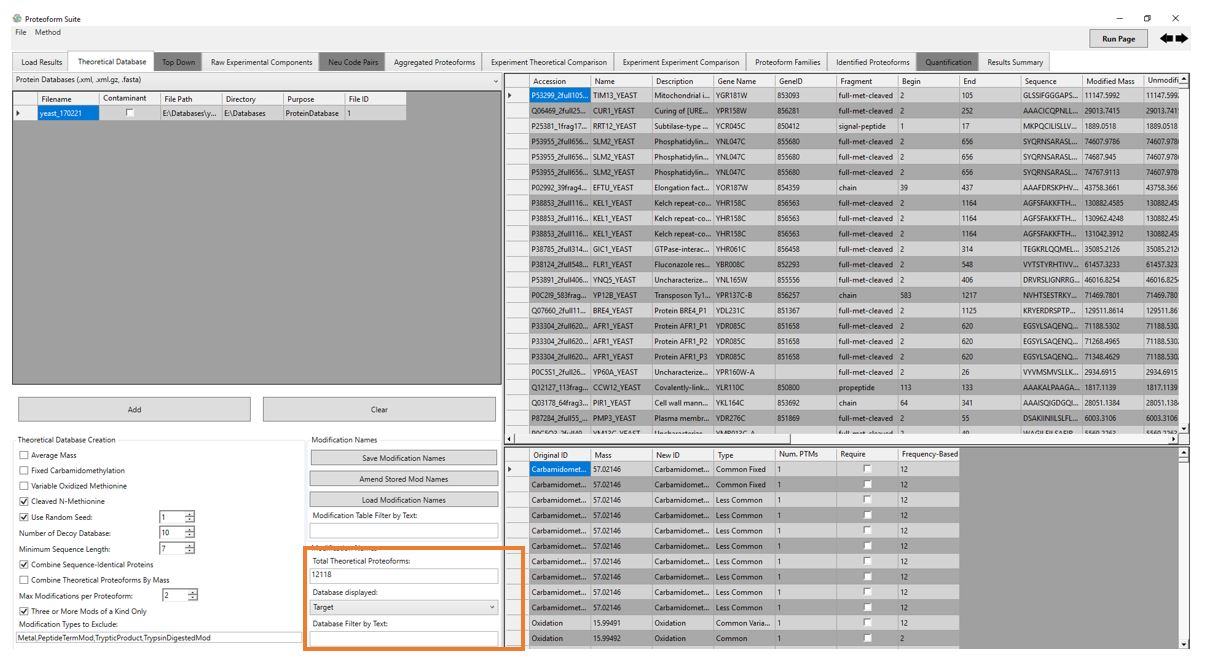
\includegraphics[scale=0.42]{figures/theoretical3.jpg}
\end{figure}
\end{itemize}
